\chapter*{Michaelis-Menten Results}
In this section, Michaelis-Menten kinetics is applied to 
the system and the results are compared with the original 
results given in the original paper.

\section*{System Description}
The system reaction is given below, which is same as the one 
given above :

\begin{center}
    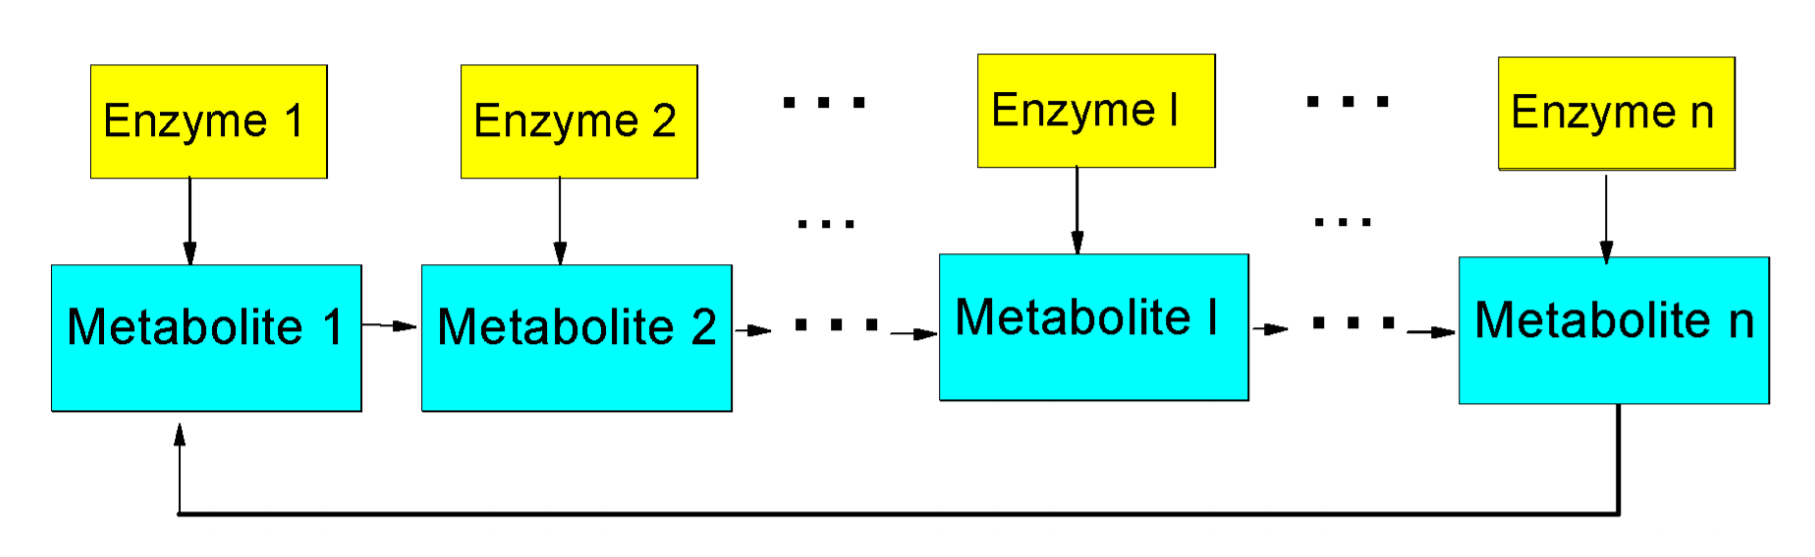
\includegraphics[scale=0.3]{img/orig-sys.png}
\end{center}

\subsection*{Rate Equations}
According to Michaelis-Menten kinetics, the rate equations 
are as given :

\begin{align*}
    \frac{d[X_i]}{dt} &= V_{\text{max}} \frac{[X_{i-1}]}{K_M + [X_{i-1}]}\\
    &= K_{i,3}[E_i]_{\text{total}} \frac{[X_{i-1}]}{\frac{K_{i,1}}{K_{i,2}} + [X_{i-1}]}\\\\
    \frac{d[E_i]}{dt} &= -K_{i,1}[E_i][X_i] + K_{i,2}[E_iX_i] + K_{i,3}[E_iX_i]\\
    &= -K_{i,1}[E_i][X_i] + (K_{i,2} + K_{i,3})\frac{[E_i]_{\text{total}}[X_i]}{K_d + [X_i]}\\\\
    \frac{d[X_iE_i]}{dt} &= k_{i,1}[X_i][E_i] - K_{i,2}[E_iX_i] + K_{i,3}[E_iX_i]\\
    &= K_{i,1}[E_i][X_i] - (K_{i,2} + K_{i,3})\frac{[E_i]_{\text{total}}[X_i]}{K_d + [X_i]}
\end{align*}

\noindent These can be further simplified, when replacing 
$[E_i]$ with $[E_i]_{\text{total}} - [X_iE_i]$. Thus the 
modified equations are :

\begin{align*}
    \frac{d[X_i]}{dt} &= K_{i,3}[E_i]_{\text{total}} \frac{[X_{i-1}]}{\frac{K_{i,1}}{K_{i,2}} + [X_{i-1}]}\\
    \frac{d[E_i]}{dt} &= -K_{i,1}[E_i]_{\text{total}}[X_i] + (K_{i,2} + K_{i,3} + [X_i])\frac{[E_i]_{\text{total}}[X_i]}{K_d + [X_i]}\\
    \frac{d[X_iE_i]}{dt} &= K_{i,1}[E_i]_{\text{total}}[X_i] - (K_{i,2} + K_{i,3} + K_{i,1}[X_i])\frac{[E_i]_{\text{total}}[X_i]}{K_d + [X_i]}
\end{align*}

\subsection*{Allosteric Binding and Negative Autoregulation}
The equations in the allosteric binding and negative 
autoregulation remain the same and thus are as follows :

\begin{align*}
    \frac{d[FP]}{dt} &= K_{rel}([FP]_{max} - [FP]) - K_{auto}[E_1]_{total}[FP]\\
    \frac{d[mRNA]}{dt} &= K_{pro}[FP] - K_d[mRNA]\\
    \frac{d[E1]_{total}}{dt} &= K_{tran}[mRNA] - K_{allo}\frac{[X_l][E_1]_{total}}{K_{half} + [E_1]_{total}}
\end{align*}

\section*{Closed Loop Systems}
Thus the rate equations for the systems are as follows :
\subsubsection*{DNA Cycle}
\begin{align*}
    \frac{d[FP]}{dt} &= K_{rel}([FP]_{max} - [FP]) - K_{auto}[E_1]_{total}[FP]\\
    \frac{d[mRNA]}{dt} &= K_{pro}[FP] - K_d[mRNA]\\
    \frac{d[E1]_{total}}{dt} &= K_{tran}[mRNA] - K_{allo}\frac{[X_l][E_1]_{total}}{K_{half} + [E_1]_{total}}
\end{align*}

\subsubsection*{Phosphorylation Cycle}

\begin{align*}
    \frac{d[X_i]}{dt} &= K_{i,3}[E_i]_{\text{total}} \frac{[X_{i-1}]}{\frac{K_{i,1}}{K_{i,2}} + [X_{i-1}]}\\
    \frac{d[X_iE_i]}{dt} &= K_{i,1}[E_i]_{\text{total}}[X_i] - (K_{i,2} + K_{i,3} + K_{i,1}[X_i])\frac{[E_i]_{\text{total}}[X_i]}{K_d + [X_i]}
\end{align*}

\subsection*{Conclusion}
Thus it can be seen that only the phosphorylation cycle has 
had any effect by changing the mechanism of calculating 
kinetics.

\section*{Analysis}
This is analysis which is done under equilibrium and various 
aspects such as robustness will be analysed.

\subsection*{Robustness}
We will use the same metric of elasticity coefficient to 
determine the robustness of the system. Thus calculation 
of $[X_l]^*$ is required which can be done by calculating 
the derivative of the latent state variable 
$[FP] + \frac{K_{rel}}{K_{pro}}[mRNA] + \frac{K_dK_{rel}}{K_{tran}K_{pro}}[E_1]_{total}$ 
which is as follows :

\begin{align*}
    &\frac{d}{dt} ([FP] + \frac{K_{rel}}{K_{pro}}[mRNA] + \frac{K_dK_{rel}}{K_{tran}K_{pro}}[E_1]_{total})\\
    =&-\frac{K_dK{rel}K_{allo}}{K_{tran}K_{pro}} \frac{[X_l][E_1]_{total}}{K_{half}+[E_1]_{total}} + K_{rel}[FP]_{max} - K_{auto}[E_1]_{total}[FP]\\
    =&-K_{gain}([X_l] - R - \frac{K_{half}[X_l]}{K_{half} + [E_1]_{total}} + \frac{K_{auto}}{K_{gain}}[E_1]_{total}[FP])
\end{align*}

It can be seen that it yields the same result and thus, from 
this, it is clear that measure of robustness will remain 
same. Thus the $[X_l]^*$ is :

\begin{align*}
    [X_l]^* &= (R - \frac{K_{auto}}{K_{gain}}[E_1]^*_{total}[FP]^*)\frac{K_{half}+[E_1]^*_{total}}{[E_1]^*_{total}}\\
    &= R(\frac{K_{rel}}{K_{auto}[E_1]^*_{total} + K_{rel}})\frac{K_{half}+[E_1]^*_{total}}{[E_1]^*_{total}}
\end{align*}

\noindent Which then leeds to the following elasticity coefficient :

\begin{equation*}
    \varepsilon = -\frac{K_{auto}[E_1]^*_{total}}{K_{auto}[E_1]^*_{total} + K_{rel}} + \frac{K_{half}}{K_{half} + [E_1]^*_{total}}
\end{equation*}

\subsection*{Conclusion}
And hence the same conclusion is drawn, which gives claim to 
the hypothesis given by the original papers' authors that it 
would remain the same.
